\scanpage{13}
% archive sheet number: 12
\deleted{\mbox{\begin{minipage}{\linewidth}
\diagram{\deleted{\mbox{\begin{tikzcd}[ampersand replacement=\&,column sep=small,row sep=large,font=\footnotesize]
d \& D(d)=\pi_0\bar\Sigma_d(\unsure{\mathfrak X|\mathscr X|\mathcal X|X})
 \arrow[r,"{\overset{\alpha_d}{\sim}}"]\arrow[d,"{R_{d',d}}"]
 \& E(d)\overset{\text{\unsure{df|dfn}}}{=}\{e\in E\mid\varphi(M(e))=d\}
 \arrow[d,"{r_{d',d}}"]\\
 \shortstack{$\cup$\\$d'$} \& D(d')\arrow[r,"{\overset{\alpha_{d'}}{\sim}}"]
 \& E(d')
\end{tikzcd}}}}

\diagram{\deleted{\mbox{\begin{tikzcd}[ampersand replacement=\&,column sep=small,row sep=small,font=\footnotesize]
D(\{i\})=\pi_0[\unsure{\deleted{\bar\Sigma}|\deleted{\Delta}\bar\Sigma}(X_i,\partial X_i)
 \arrow[r,"{\overset{\alpha_i}{\sim}}"]
 \& E(\{i\})=\varphi^{-1}(\{i\})\\
 \begin{array}{cc}\Vert&\backslash\\[-2pt]
 \displaystyle\bigcup_{\mu\varphi(M(e))\le i}|E_e|,
 &\displaystyle\bigcup_{\mu\varphi\unsure{\lvert|(}M(e)<i}(E_e\rvert
 \end{array} \&
\end{tikzcd}}}}

\[
\deleted{\partial X_i=\bigcup_{\mu(\varphi(M(e)))<i}|E_e|}
\]
\[
\deleted{\partial X_i\overset{\text{\unsure{df|dfn}}}{=}\bigcup_{j<i}X_j
 =\bigcup_{j<i}\ \bigcup_{\substack{e\in E\\\varphi M e)\le j}}|E_e|
 =\bigcup_{\substack{e\in E\\\exists\,j\ \text{tel que}\\\varphi\mathord{.}(M\mathord{.}(e))\le j<i}}|E_e|}
\]
\figure{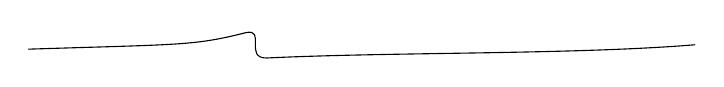
\begin{tikzpicture}[x=0.7cm,y=0.7cm]
\draw (0,0) .. controls (2.8,0.09) and (3.0,0.06) .. (3.95,0.30)
 .. controls (4.32,0.38) and (3.91,-0.17) .. (4.33,-0.16)
 .. controls (6.6,-0.05) and (9.9,-0.10) .. (12.1,0.08);
\end{tikzpicture}}

\[
\deleted{|\unsure{\mathcal K|K|k}|=(K_0,K)\supset(L_0,L)=|L|}
\qquad\mathrel{.\mkern2mu:}
\]
\[
\deleted{\bar\Sigma\overset{\substack{\deleted{\unsure{\alpha|\Delta|A|x}}\\\downarrow\\\deleted{\unsure{X|K}}}}{(}|K|,|L|)=|\Delta|}
\]
\[
\deleted{\widetilde{\unsure{\deleted{K}\Delta|\deleted{\Delta}K}}\overset{\text{\unsure{df|dfn}}}{=}
 \Sigma(K,L)=(\widetilde{\unsure{\deleted{K}\Delta|\deleted{\Delta}K}}_0,\widetilde{\unsure{\deleted{K}\Delta|\deleted{\Delta}K}})}
\]
\[
\deleted{\left\{\begin{aligned}
 \widetilde{\unsure{\deleted{K}\Delta|\deleted{\Delta}K}}_0&=\varinjlim_{\sigma\in K\setminus L}
 \underset{\cdot}{\sigma}\;(\subset{\unsure{\deleted{\Delta}K|\deleted{K}\Delta}}_0)\xrightarrow{\unsure{\pi|\bar\pi}}{\unsure{\deleted{\Delta}K|\deleted{K}\Delta}}_0\\
 \widetilde{\unsure{\deleted{K}\Delta|\deleted{\Delta}K}}&=\mathrm{Im}\bigl((K\setminus L)\longrightarrow
 \mathcal P(\Delta_0)\bigr)
\end{aligned}\right.}
\]

\diagram{\deleted{\mbox{\begin{tikzcd}[ampersand replacement=\&,row sep=small,column sep=small]
 \deleted{\unsure{\bar\Sigma|\Sigma|E}}|\widetilde{\unsure{\deleted{K}\Delta|\deleted{\Delta}K}}|\arrow[r,"?"]
 \& \Sigma(|K|,|L|)\\
 \Vert \& \sigma'=\mathrm{Im}(\sigma) \& \underline{\sigma}\in K\setminus L\\
 \displaystyle\varinjlim_{\sigma'\in\Delta}|\sigma'| \&
 |\sigma|\arrow[r]\arrow[rr,bend right=12] \& |\sigma'|\arrow[r] \& \Sigma
\end{tikzcd}}}}
\end{minipage}}}
